\section{Experiments}\label{sec:experiments}

In this section, we empirically validate the effectiveness of \sname. Specifically, in $\S$~\ref{subsec:main_result}, we present quantitative and qualitative comparisons against existing autonomous research agents. In $\S$~\ref{subsec:ablation}, we conduct component-wise ablation studies to evaluate each constituent part of \sname. In $\S$~\ref{subsec:discussion}, we provide a discussion including cost analysis and case studies.

\noindent\textbf{Common Setup.} We evaluate the effectiveness of \sname\ on 107 scientific problems drawn from top machine learning venues, including ICLR, ICML, and NeurIPS (see Appendix~\ref{subapp:benchmark} for details). All experiments are conducted using Gemini 3.6 Flash and Claude Opus 4.8, unless otherwise specified. For evaluation, we primarily report review scores from automated AI review agents: ScholarPeer \citep{goyal2026scholarpeer} and Stanford Agentic Reviewer\footnote{\url{https://paperreview.ai/}}. ScholarPeer serves as an in-distribution evaluation, as it is also used to refine the draft quality generated by \sname. Conversely, Stanford Agentic Reviewer serves as a held-out evaluator that was unseen during development by both the baselines and our method. Full implementation details and configurations are provided in Appendix~\ref{subapp:config}.

\subsection{Main Results}\label{subsec:main_result}
\begin{table}[t!]
\centering
\caption{\textbf{Comparison with autonomous research agents.} We report the average review ratings, standard deviations (1--10 scale), and acceptance rates (\%) given by ScholarPeer and Stanford Agentic Reviewer. The column ``\# Papers'' represents the number of publicly released AI-generated papers by each autonomous research agent used to aggregate performance. Bold indicates the best performance.}\label{tab:vs_ai_scientist}
\begin{tabular}{lccccc}
\toprule
& & \multicolumn{2}{c}{\textbf{ScholarPeer}} & \multicolumn{2}{c}{\textbf{Stanford Agentic Reviewer}}\\
\cmidrule(lr){3-4}\cmidrule(lr){5-6}
\textbf{Framework} & \textbf{\# Papers} & \multicolumn{1}{c}{\textbf{Avg. Rating}} & \multicolumn{1}{c}{\textbf{Accept Rate}} & \multicolumn{1}{c}{\textbf{Avg. Rating}} & \multicolumn{1}{c}{\textbf{Accept Rate}}\\
\midrule
AI-Researcher & \phantom{0}7 & 1.0\stdv{0.0} & \phantom{0}0.0 & 2.4\stdv{0.6} & \phantom{0}0.0\\
CycleResearcher & \phantom{0}6 & 1.0\stdv{0.0} & \phantom{0}0.0 & 2.8\stdv{1.0} & \phantom{0}0.0\\
AI Scientist-v2 & \phantom{0}3 & 2.0\stdv{1.0} & \phantom{0}0.0 & 2.5\stdv{0.2} & \phantom{0}0.0\\
AutoResearchClaw & \phantom{0}4 & 2.5\stdv{1.0} & \phantom{0}0.0 & 3.7\stdv{0.5} & \phantom{0}0.0\\
Zochi & \phantom{0}2 & 3.0\stdv{0.0} & \phantom{0}0.0 & 2.9\stdv{0.6} & \phantom{0}0.0\\
DeepScientist & \phantom{0}3 & 3.0\stdv{0.0} & \phantom{0}0.0 & 4.1\stdv{0.6} & \phantom{0}0.0\\
ScientistOne & 21 & 3.8\stdv{1.2} & 14.3 & 4.1\stdv{0.7} & \phantom{0}0.0\\
\rowcolor{Gray}\textbf{\sname~(Ours)} & 86 & \textbf{7.5}\stdv{1.3} & \textbf{91.9} & \textbf{5.7}\stdv{0.6} & \textbf{72.1} \\
\bottomrule
\end{tabular}
\end{table}
\noindent\textbf{Quantitative Comparison.} As shown in Table~\ref{tab:vs_ai_scientist}, \sname~achieves a 91.9\% acceptance rate under ScholarPeer (nearly doubling the review score from ScientistOne's 3.8 to 7.5). More importantly, while all baselines fail to achieve acceptance from the Stanford Agentic Reviewer, \sname~is the only agent that produces research where 72.1\% of generated papers meet high acceptance standards. This result shows that while current autonomous research agents cannot produce expert-level research results, \sname~possesses such capabilities.

\begin{figure*}[t!]
  \centering
  \setlength{\tabcolsep}{0pt} 
  \renewcommand{\arraystretch}{0}
  \resizebox{\textwidth}{!}{
  \begin{tabular}{|c|c|c|}
  \hline
    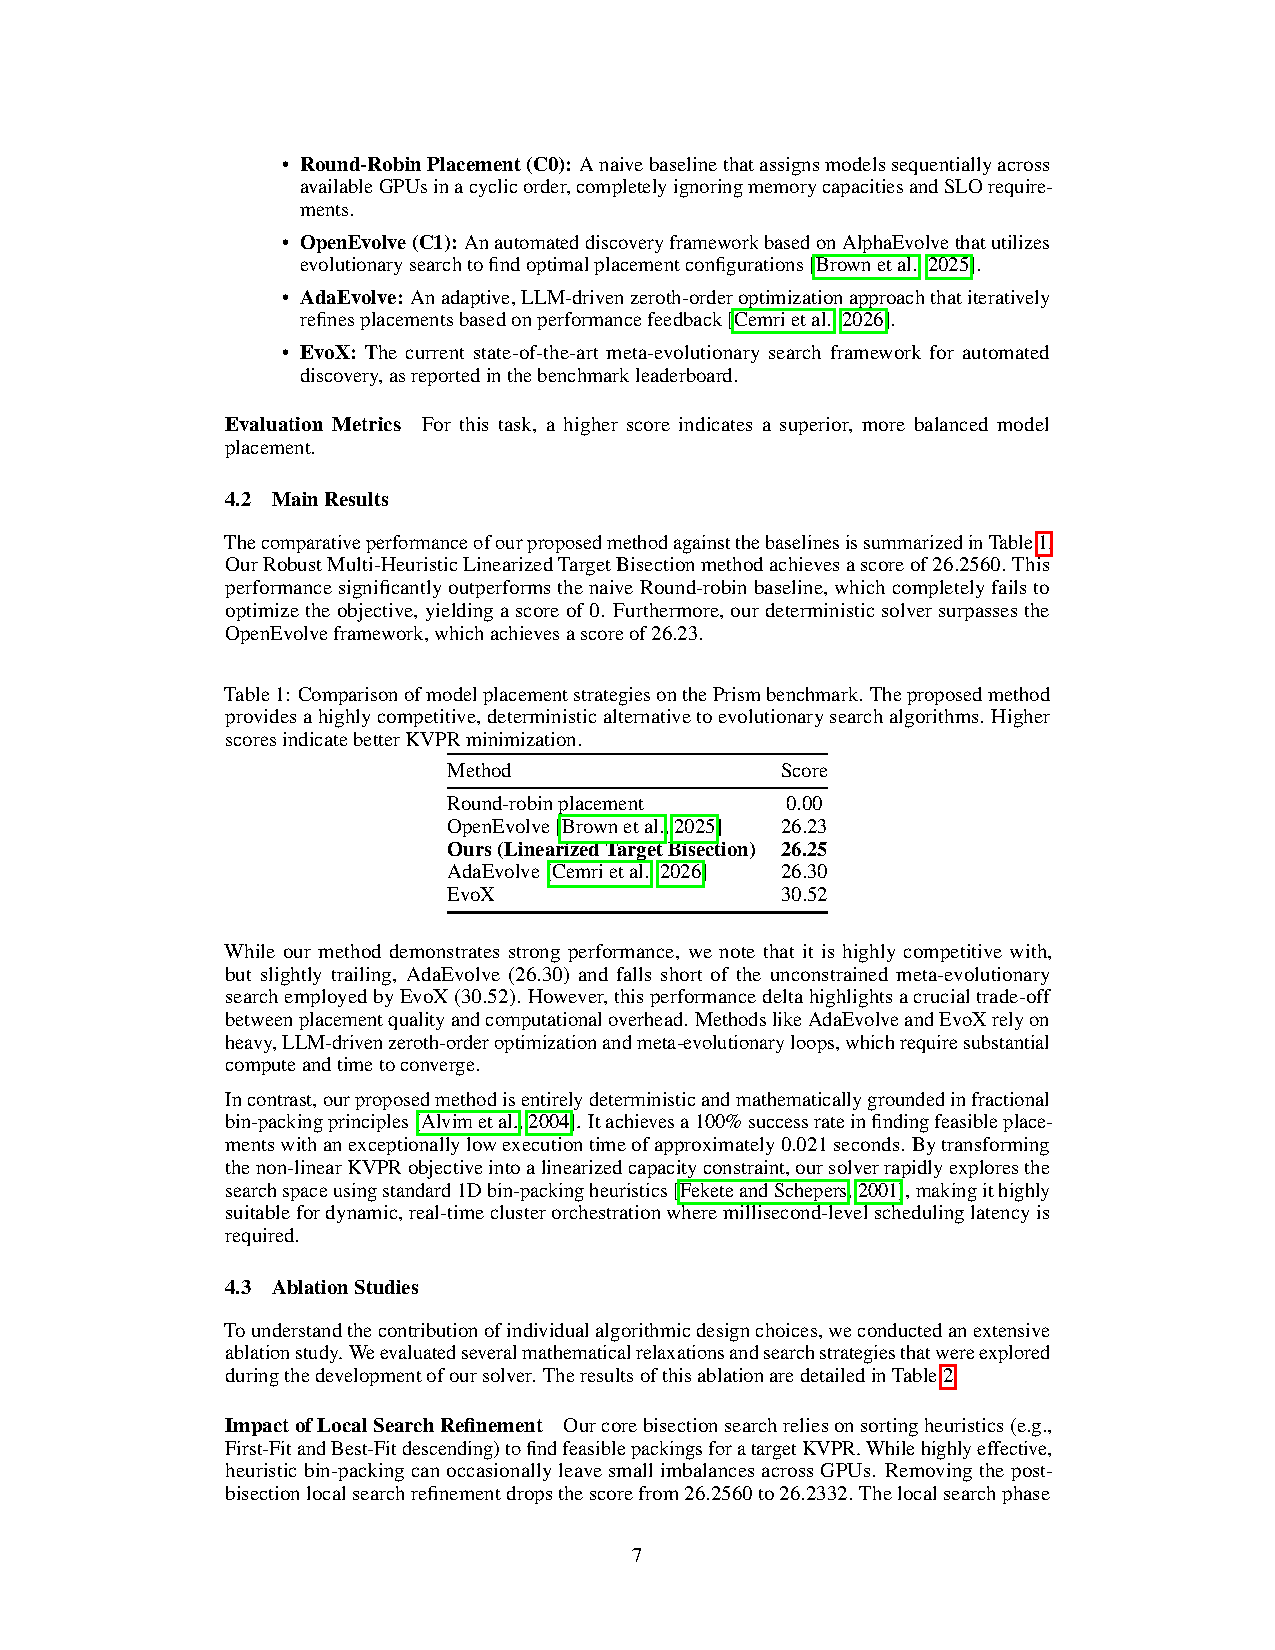
\includegraphics[width=0.2\textwidth]{figures/compare_pdfs/scientistone_7.pdf} &
    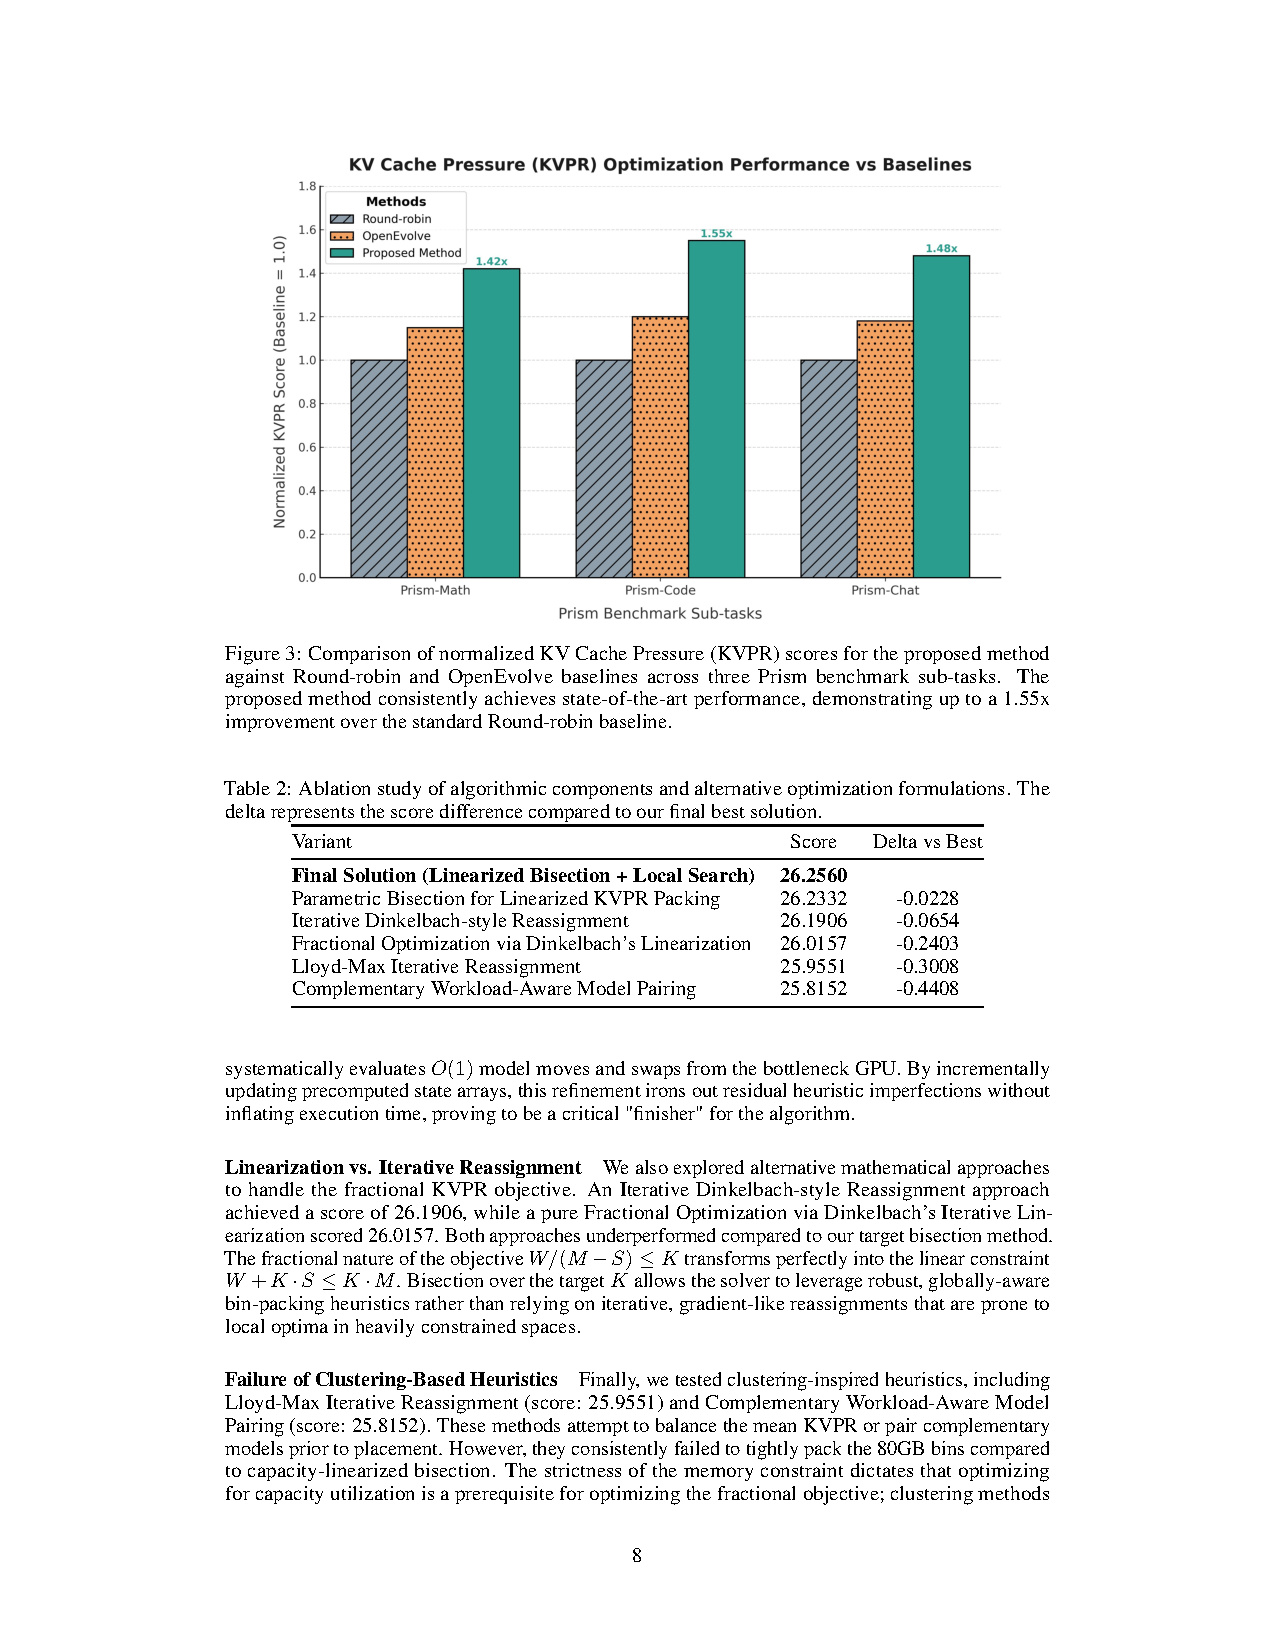
\includegraphics[width=0.2\textwidth]{figures/compare_pdfs/scientistone_8.pdf} &
    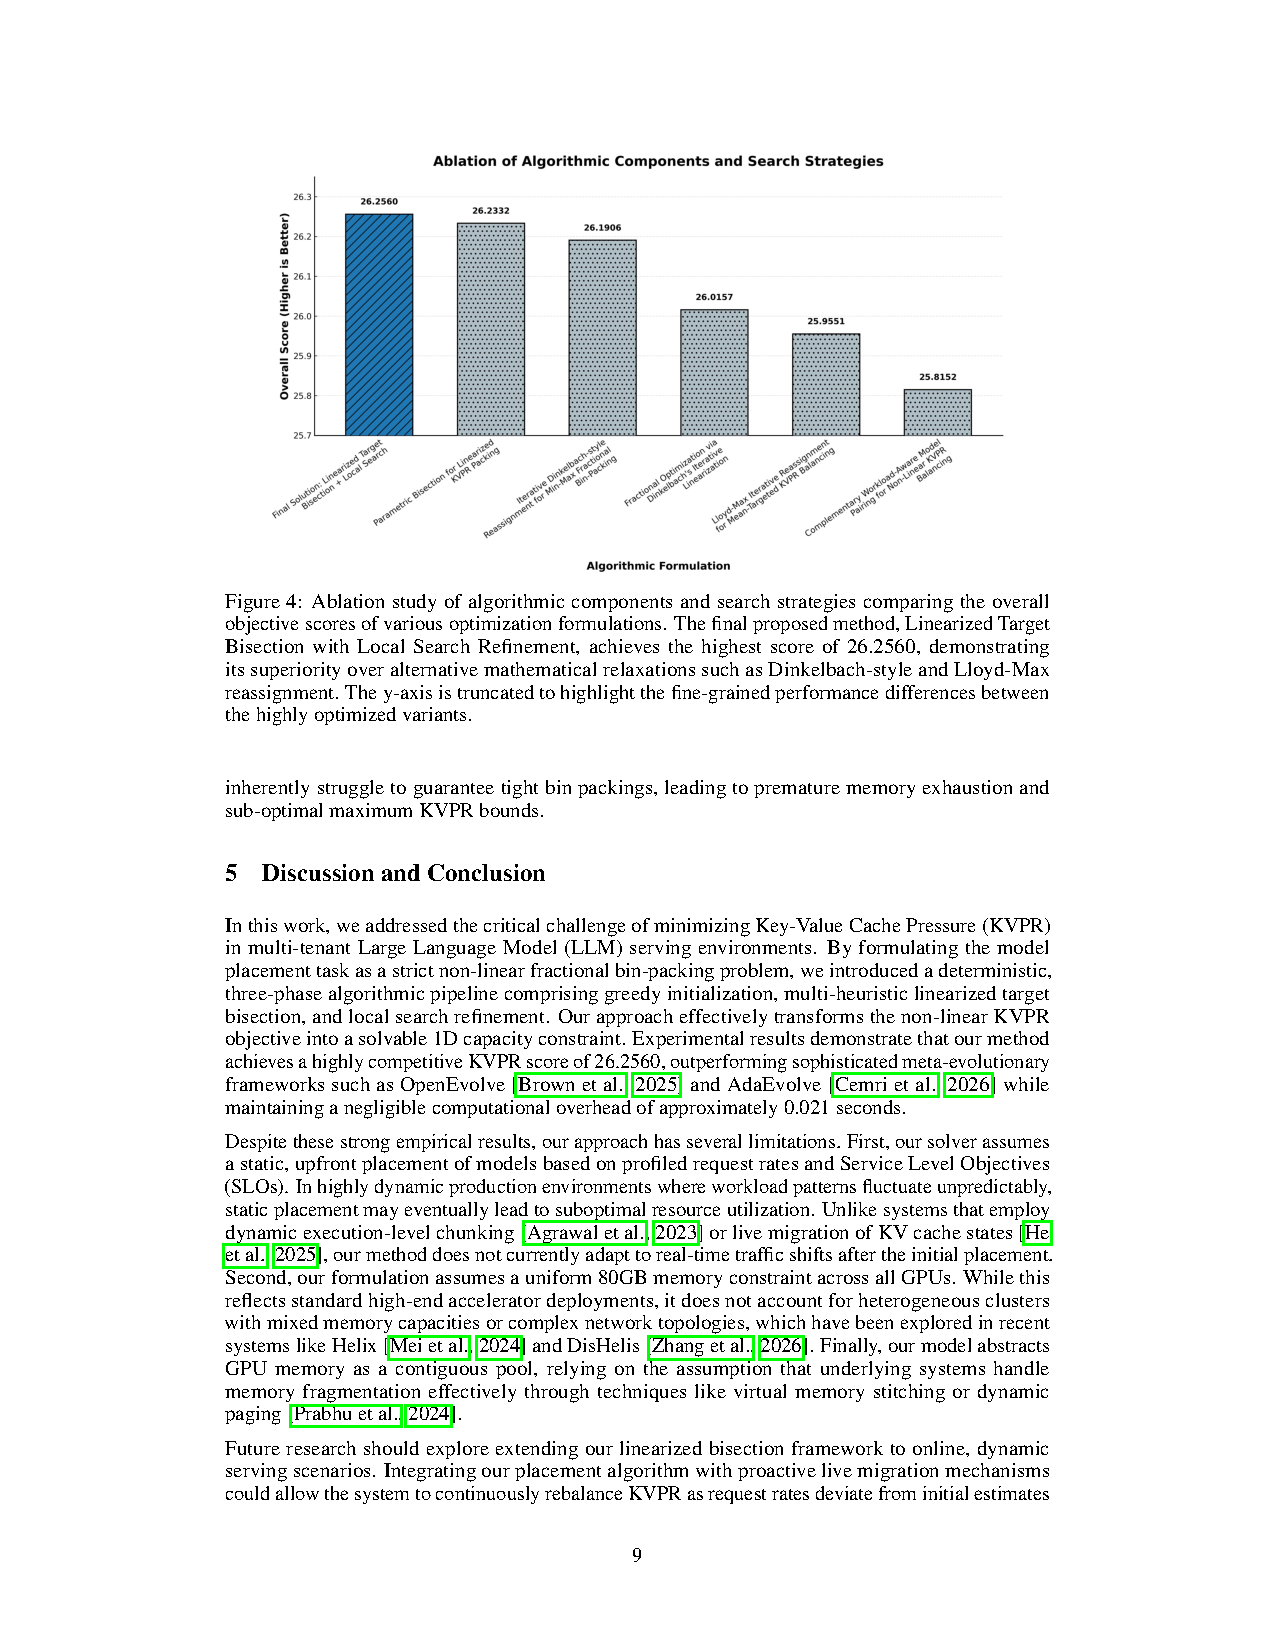
\includegraphics[width=0.2\textwidth]{figures/compare_pdfs/scientistone_9.pdf}\\
    \hline
    \multicolumn{3}{c}{\tiny{\phantom{0}}}\\
    \multicolumn{3}{c}{\tiny{(a) Experiment section generated by ScientistOne \citep{meng2026scientistone}}}\\
    \multicolumn{3}{c}{\tiny{\phantom{0}}}\\
    \hline
    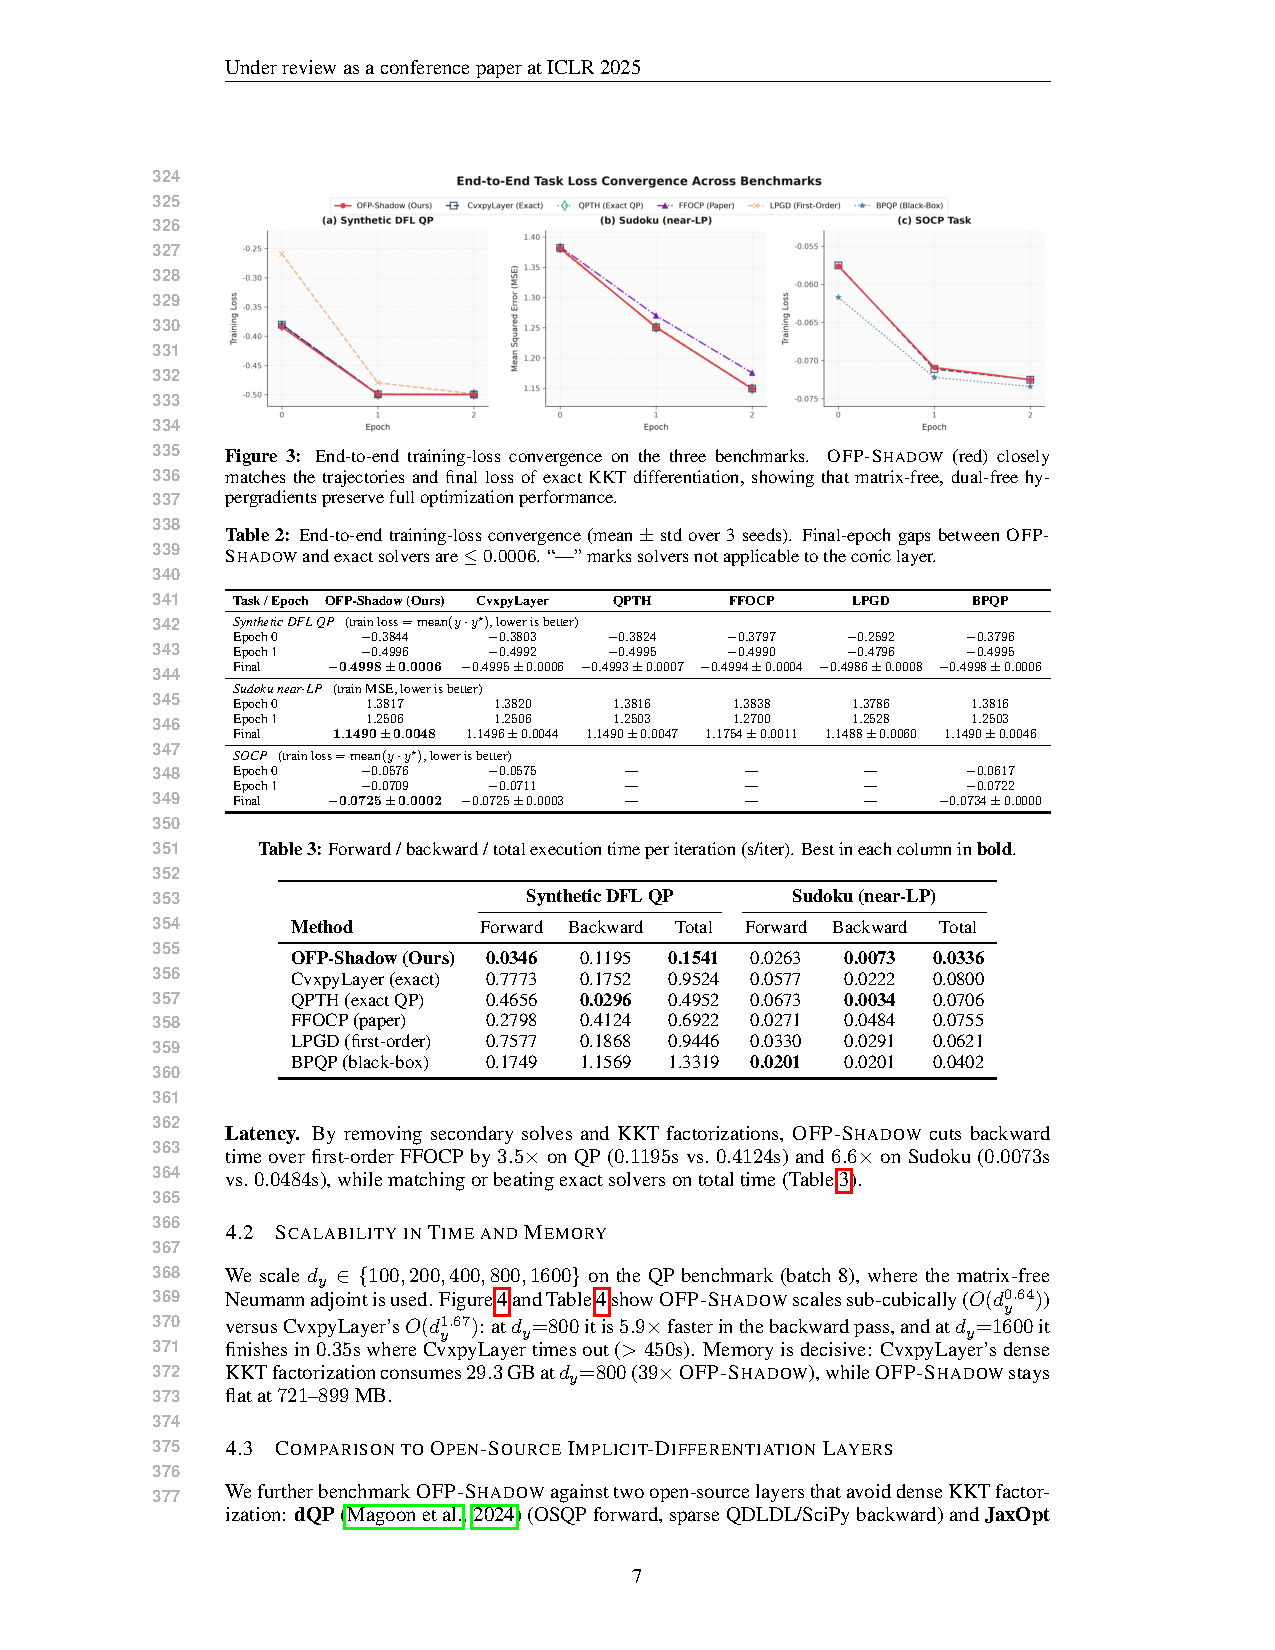
\includegraphics[width=0.2\textwidth]{figures/compare_pdfs/ours_7.pdf} &
    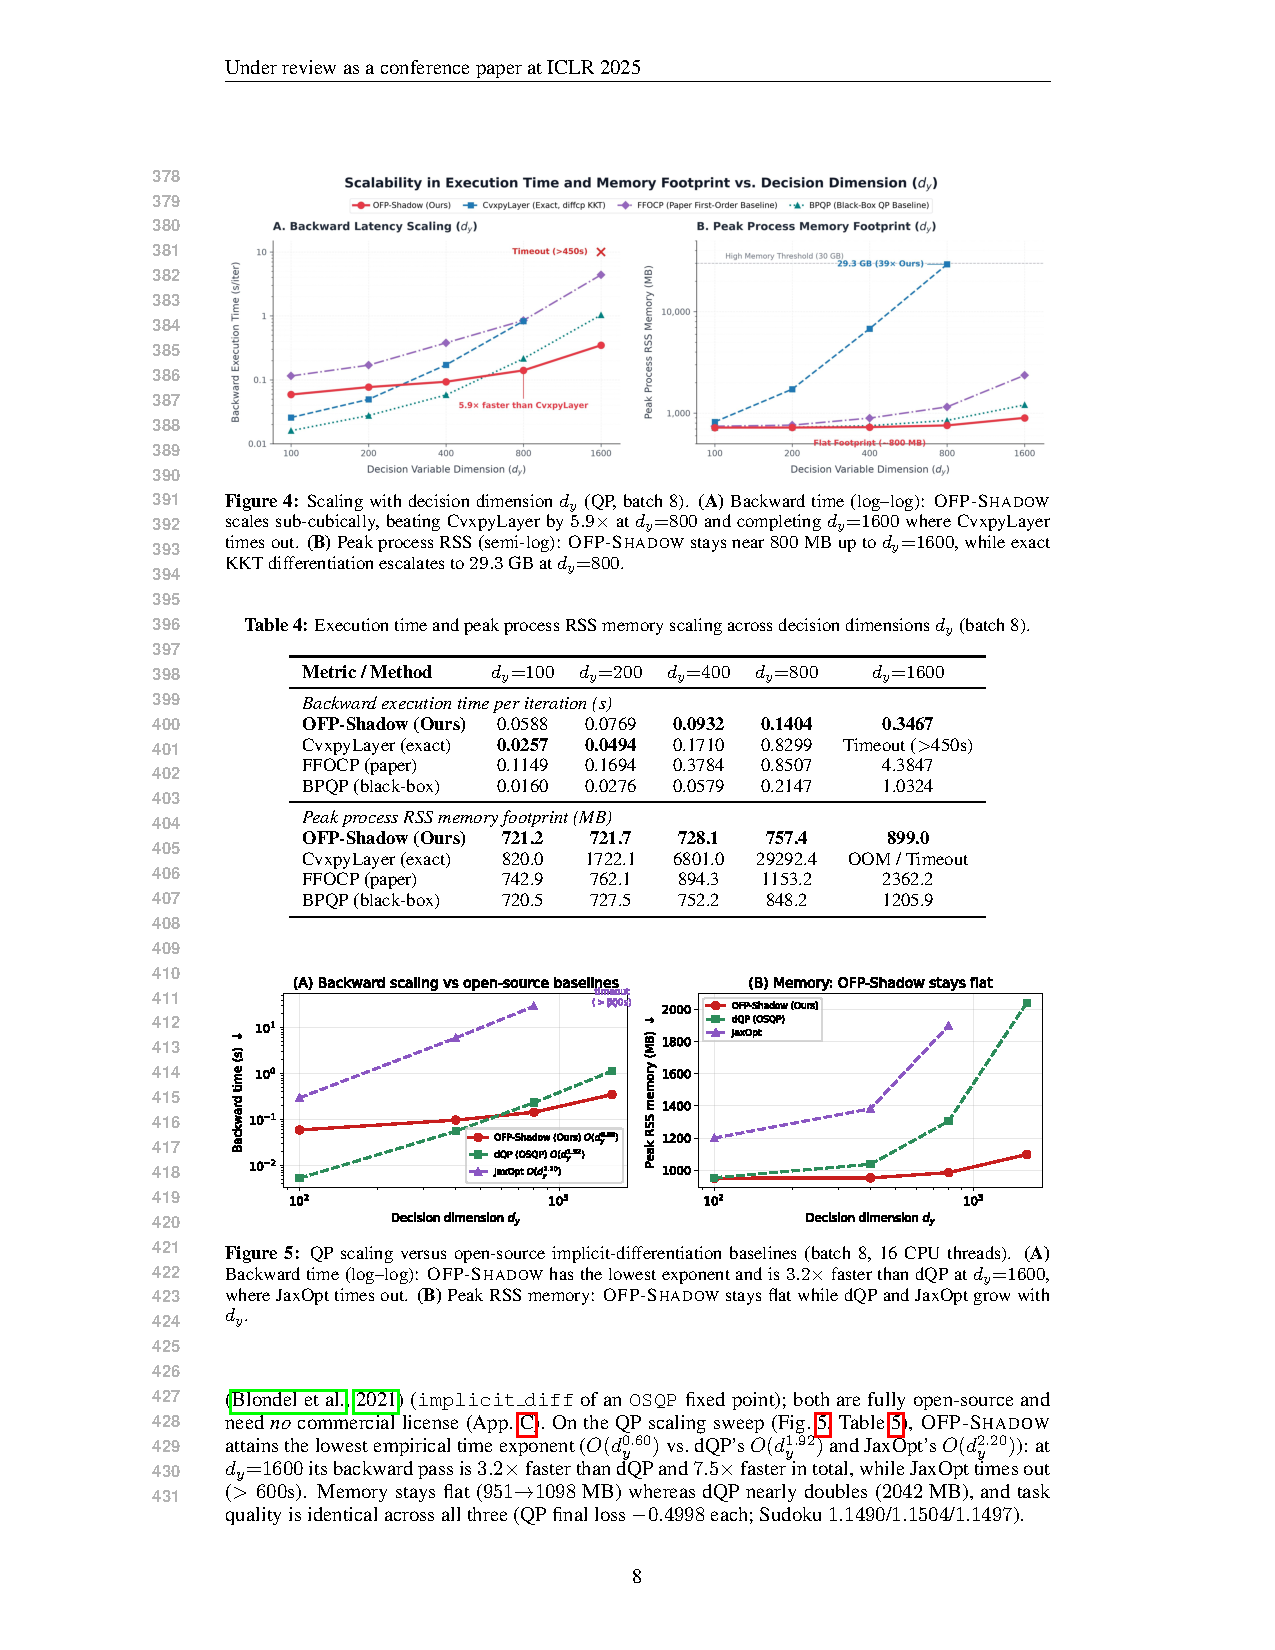
\includegraphics[width=0.2\textwidth]{figures/compare_pdfs/ours_8.pdf} &
    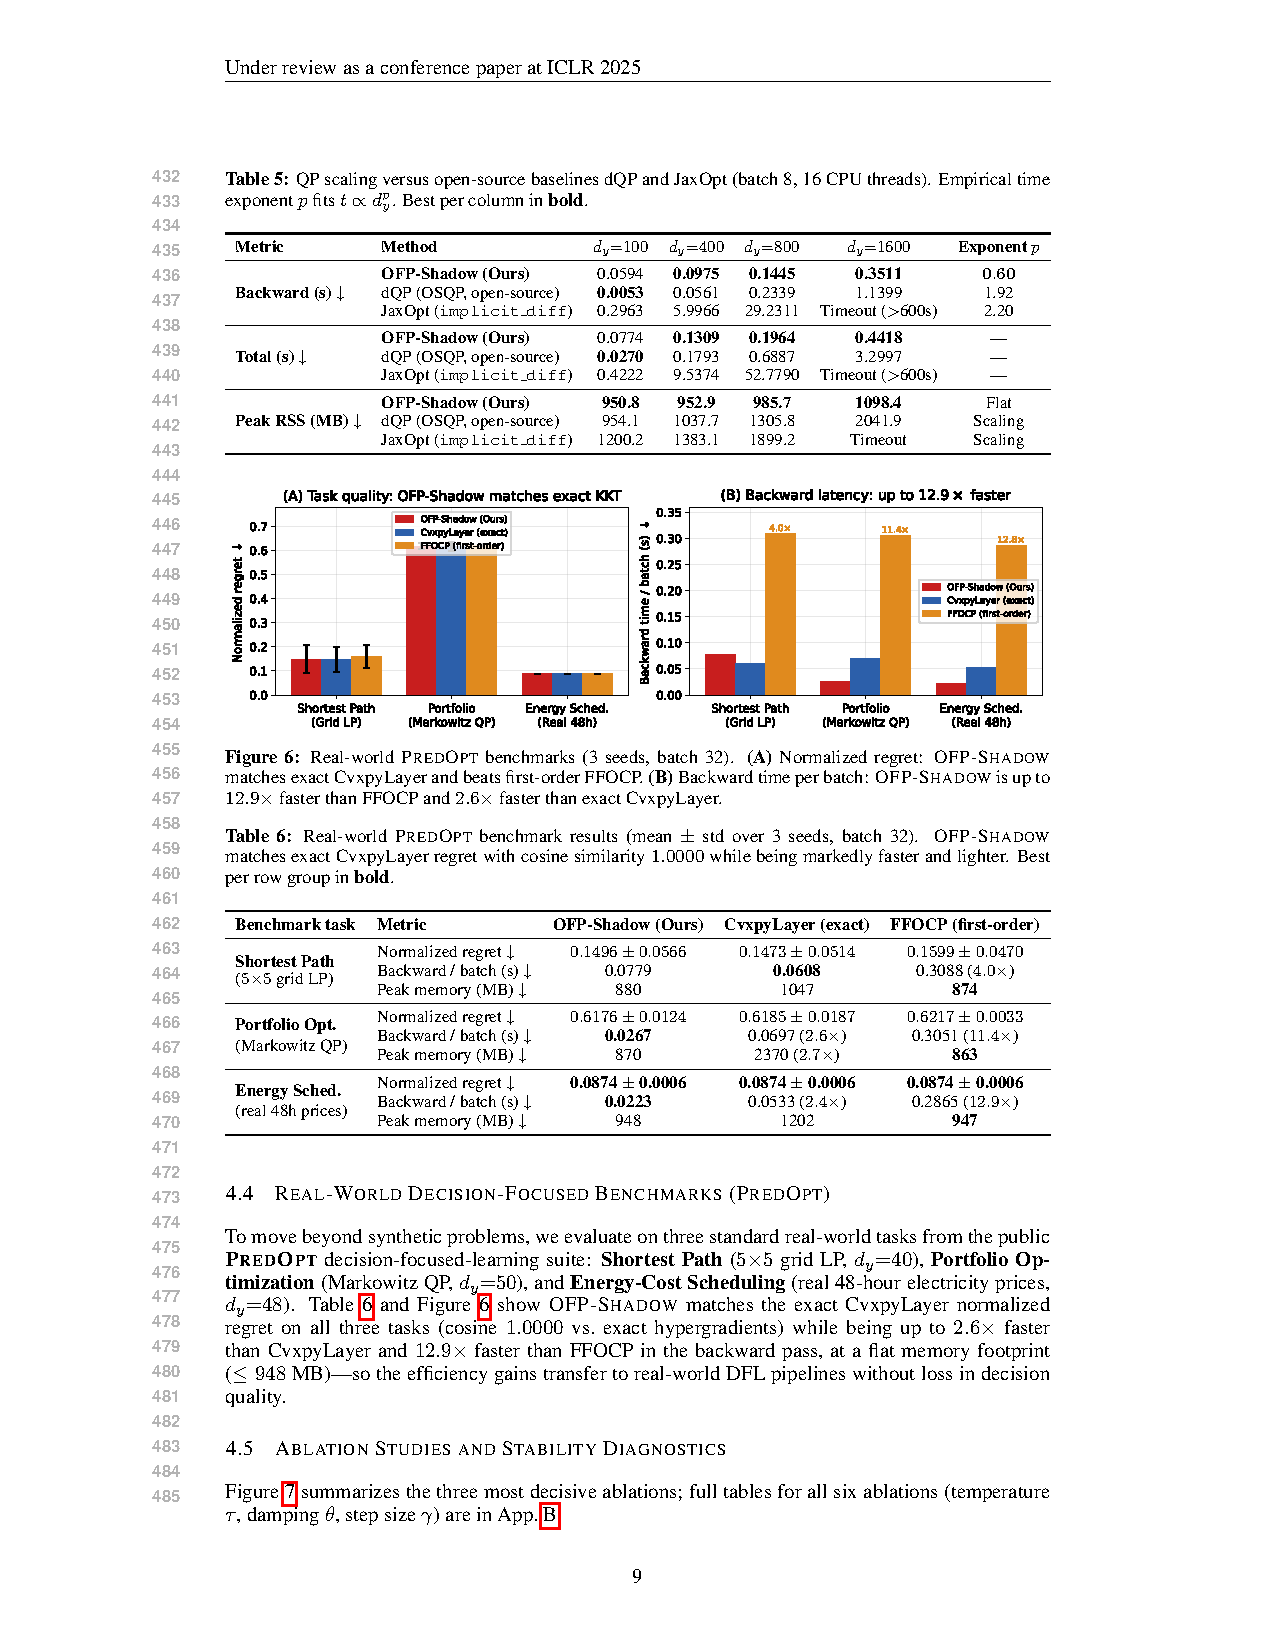
\includegraphics[width=0.2\textwidth]{figures/compare_pdfs/ours_9.pdf}\\
    \hline
     \multicolumn{3}{c}{\tiny{\phantom{0}}}\\
    \multicolumn{3}{c}{\tiny{(b) Experiment section generated by \textbf{\sname~(Ours)}}}\\
  \end{tabular}}
  \caption{\textbf{Qualitative comparison.} Side-by-side comparison of the experiment section generated by \sname~against the highest-reviewed paper from ScientistOne \citep{meng2026scientistone}.}
  \label{fig:qual_compare_main}
\end{figure*}
\noindent\textbf{Qualitative Comparison.}
To assess the depth and completeness of the generated manuscripts, we compare \sname~against the strongest baseline, ScientistOne. As illustrated in Figure~\ref{fig:qual_compare_main}, \sname~demonstrates substantially broader experimental coverage and analytical rigor. While ScientistOne generates only 4 figures and 2 tables—evaluating a single metric on an isolated benchmark with limited baselines—\sname~produces 9 figures and 12 tables (including the Appendix). Furthermore, \sname~reports multi-metric evaluations across diverse datasets and incorporates an extensive set of baseline comparisons, reflecting a publication-ready experimental design.

\begin{table}[t!]
\centering
\caption{\textbf{Comparison with human-author papers and AI-generated papers.} We report the average review ratings, standard deviations (1--10 scale), and  acceptance rates (\%) evaluated by ScholarPeer \citep{goyal2026scholarpeer} and Stanford Agentic Reviewer. The top section evaluates papers accepted at each venue, which serve as inputs for \sname. The bottom section reports the evaluation of papers generated by \sname~using the accepted papers from the corresponding venue. The column ``\# Papers'' indicates the number of accepted reference papers evaluated or the number of papers successfully generated by \sname. $\dagger$ denotes AI-generated papers.}\label{tab:vs_conference}
% \vspace{-0.1in}
\resizebox{\textwidth}{!}{
\begin{tabular}{lccccc}
\toprule
& & \multicolumn{2}{c}{\textbf{ScholarPeer}} & \multicolumn{2}{c}{\textbf{Stanford Agentic Reviewer}}\\
\cmidrule(lr){3-4}\cmidrule(lr){5-6}
\textbf{Venue} & \textbf{\# Papers} & \multicolumn{1}{c}{\textbf{Avg. Rating}} & \multicolumn{1}{c}{\textbf{Accept Rate}} & \multicolumn{1}{c}{\textbf{Avg. Rating}} & \multicolumn{1}{c}{\textbf{Accept Rate}}\\
\midrule
Agent4Science 2025 Accepted$^\dagger$ & \phantom{0}4 & 3.0\stdv{0.0} & \phantom{0}\phantom{0}0.0 & 3.8\stdv{0.4} & \phantom{0}0.0\\
ICLR 2026 Accepted & \phantom{0}5 & 6.8\stdv{1.6} & \phantom{0}60.0 & 5.2\stdv{0.7} & 60.0 \\
NeurIPS 2025 Accepted & 38 & 6.2\stdv{1.9} & \phantom{0}65.8 & 5.5\stdv{0.7} & 76.3 \\
ICML 2026 Spotlight & 64 & 6.9\stdv{1.5} & \phantom{0}79.7 & 6.1\stdv{0.5} & 96.9 \\
\midrule
\rowcolor{Gray}\textbf{\textit{\sname~(Ours)}} & & & & & \\
\midrule
ICLR 2026$^\dagger$ & \phantom{0}4/5\phantom{00} & 7.0\stdv{1.2} & 100.0 & 5.4\stdv{0.2} & 75.0 \\
NeurIPS 2025$^\dagger$ & 33/38\phantom{0} & 7.3\stdv{1.7} & \phantom{0}87.9 & 5.6\stdv{0.7} & 75.8 \\
ICML 2026 Spotlight$^\dagger$ & 49/64\phantom{0} & 7.6\stdv{1.0} & \phantom{0}93.9 & 5.7\stdv{0.6} & 69.4 \\
Overall$^\dagger$ & 86/107 & 7.5\stdv{1.3} & \phantom{0}91.9 & 5.7\stdv{0.6} & 72.1 \\
\bottomrule
\end{tabular}}
\end{table}
\noindent\textbf{Comparison with Human Researchers.} We evaluate the research quality produced by \sname~against accepted publications. Specifically, we use ScholarPeer and the Stanford Agentic Reviewer to evaluate papers accepted at NeurIPS 2025, ICLR 2026, and ICML 2026 (including spotlight presentations), whose problem specifications and codebases serve as benchmark tasks for \sname. As shown in Table~\ref{tab:vs_conference}, \sname~successfully executes research on 86 out of 107 problems, achieving an 80.4\% success rate. Furthermore, papers generated by \sname~surpass the average scores of accepted papers at ICLR 2026 and NeurIPS 2025 under both ScholarPeer and Stanford Agentic Reviewer. While \sname~does not yet achieve spotlight-level quality, these results still demonstrate that it functions as an expert-level research agent capable of producing manuscripts that meet the acceptance threshold of top-tier AI venues. Finally, we include comparisons with AI-generated papers accepted at Agent4Science 2025—the first venue dedicated to AI-generated research—to demonstrate that prior systems were incapable of meeting top conference standards.

\begin{table}[t!]
\centering
\caption{\textbf{Comparison with AutoSOTA.} We report the number of tasks successfully done by each framework, and performance gain (\%) across successful cases. For NeurIPS 2025 and ICLR 2026, evaluations use the same set of 33 and 4 input papers, respectively. Bold indicates the best score.}\label{tab:vs_autosota}
% \vspace{-0.1in}
\resizebox{\textwidth}{!}{
\begin{tabular}{lccccccc}
\toprule
& \multicolumn{3}{c}{\textbf{Overall}} & \multicolumn{2}{c}{\textbf{NeurIPS 2025}} & \multicolumn{2}{c}{\textbf{ICLR 2026}}\\
\cmidrule(lr){2-4}\cmidrule(lr){5-6}\cmidrule(lr){7-8}
\textbf{Framework} & \multicolumn{1}{c}{\textbf{\# Papers}} & \multicolumn{1}{c}{\textbf{Med. Gain}} & \multicolumn{1}{c}{\textbf{Avg. Gain}} & \multicolumn{1}{c}{\textbf{Med. Gain}} & \multicolumn{1}{c}{\textbf{Avg. Gain}} & \multicolumn{1}{c}{\textbf{Med. Gain}} & \multicolumn{1}{c}{\textbf{Avg. Gain}} \\
\midrule
AutoSOTA \citep{li2026autosota} & 105 & 2.7 & \phantom{0}7.5 & 3.7 & \phantom{0}8.5 & \textbf{5.0} & \textbf{7.2}\\
\rowcolor{Gray}\textbf{\sname~(Ours)} & \phantom{0}86 & \textbf{7.7} & \textbf{25.2} & \textbf{7.0} & \textbf{13.9} & 2.2 & 3.8 \\
\bottomrule
\end{tabular}}
\end{table}
\noindent\textbf{Comparison with AutoSOTA.} While AutoSOTA~\citep{li2026autosota} operates in a distinct setting, i.e., modifying existing codebases to optimize a single scalar metric, \sname~is designed for end-to-end scientific paper generation. For completeness, we provide a comparison based on the performance gains reported over human state-of-the-art baselines. To extract these gains systematically, we parse the main tables for 10 times using Gemini 3.6 Flash and averaged them. As shown in Table~\ref{tab:vs_autosota}, \sname~shows superior performance to AutoSOTA in terms of average and median improvement across average of all tasks and NeurIPS 2025 tasks, but performance drops slightly in the ICLR 2026 tasks.
% Furthermore, across the shared benchmark of 33 NeurIPS 2025 papers, \sname~demonstrates a markedly stronger ability to advance the empirical frontier. 
We hypothesize that this advantage stems from \sname~proposing novel methodological innovations to overcome baseline limitations, whereas AutoSOTA relies primarily on searching within the existing hyperparameter and execution space to improve the given method. Appendix~\ref{sec:autosota} examines the five ICLR 2026 papers one by one and supports this account: none of AutoSOTA's five changes introduces a new algorithmic component, and each is a configuration-level edit of at most a few lines.

\subsection{Ablation Studies}\label{subsec:ablation}

Here, we evaluate on the 49 target problems sourced from ICML 2026 Spotlight papers.

\begin{figure}[t!]
\centering
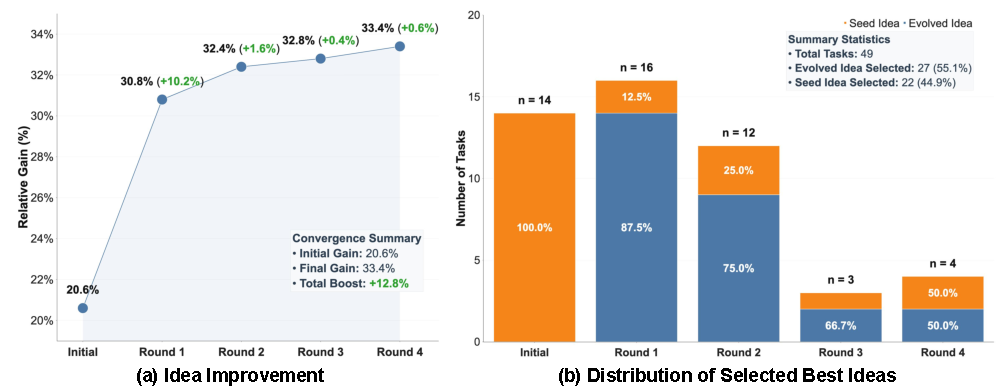
\includegraphics[width=\linewidth]{figures/scientisttwo_idea_improvement_ablation.pdf}
\caption{\textbf{Ablation on idea improvement.} \textbf{(a)} Relative performance gains are largest during the initial improvement rounds and steadily diminish in later stages.
\textbf{(b)} Top-performing ideas emerge early in the refinement process. Across iterations, evolved ideas are selected for the majority of tasks.}
\label{fig:abl_idea_improvement}
\end{figure}
\noindent\textbf{Effectiveness of Idea Evolution.} As shown in Figure~\ref{fig:abl_idea_improvement}(a), the relative gain over the human state-of-the-art baseline steadily increases as \sname~proceeds through iterative idea refinement. In particular, the magnitude of improvement is most pronounced during the early refinement stages.

\noindent\textbf{Balancing Exploration and Exploitation.} As shown in Figure~\ref{fig:abl_idea_improvement}(b), the majority of the top-performing ideas chosen by the Selector Agent are identified in the early stages. This indicates that the initial seed ideas generated by \sname~to overcome the limitations of human state-of-the-art methods are already well-formed and competitive. Conversely, when seed ideas yield marginal gains or fail, the Idea Evolver Agent leverages these experimental traces to evolve them into stronger hypotheses that overcome baseline shortcomings. Consequently, as refinement progresses, newly selected best ideas are substantially more likely to be drawn from evolved candidates rather than original seed ideas (as evidenced by the dominant share of the blue bars after the initial round).

\begin{table}[t!]
\centering
\caption{\textbf{Effectiveness of peer-review simulation.} Average review ratings (1--10 scale) and acceptance rates (\%) evaluated by ScholarPeer and Stanford Agentic Reviewer. Best score is bolded.}\label{tab:abl_rebuttal}
\resizebox{\textwidth}{!}{
\begin{tabular}{lcccccc}
\toprule
& & & \multicolumn{2}{c}{\textbf{ScholarPeer}} & \multicolumn{2}{c}{\textbf{Stanford Agentic Reviewer}}\\
\cmidrule(lr){4-5}\cmidrule(lr){6-7}
\textbf{Framework} & \textbf{Review Round} & \textbf{Rebuttal Agent} & \textbf{Avg. Rating} & \textbf{Accept Rate} & \textbf{Avg. Rating} & \textbf{Accept Rate} \\
\midrule
ScientistOne & - & - & 3.8\stdv{1.2} & 14.3 & 4.1\stdv{0.7} & \phantom{0}0.0 \\
\sname~(Variant) & 0 & \textcolor{Red}{\ding{55}} & 5.2\stdv{2.2} & 46.9 & 5.6\stdv{0.5} & 49.0  \\
\sname~(Ours) & 1 & \textcolor{Green}{\ding{51}} & 6.9\stdv{1.6} & 79.6 & \textbf{5.8}\stdv{0.6} & \textbf{73.5}  \\
\rowcolor{Gray}\textbf{\sname~(Ours)} & 2 & \textcolor{Green}{\ding{51}} & \textbf{7.6}\stdv{1.0} & \textbf{93.9} & 5.7\stdv{0.6} & 69.4  \\
\bottomrule
\end{tabular}}
\end{table}
\noindent\textbf{Effectiveness of the Rebuttal Agent.} During the simulated dynamic peer-review phase, \sname~leverages the Rebuttal Agent to conduct supplementary experiments and uses the findings to enhance the draft. As shown in Table~\ref{tab:abl_rebuttal}, this rebuttal procedure effectively addresses the weaknesses flagged by ScholarPeer.
While it is not surprising that \sname~gradually achieves good scores on ScholarPeer, as we utilize ScholarPeer reviews, we found that our peer-review simulation framework is generalized across Review Agent. Specifically, incorporating ScholarPeer reviews also improves acceptance rate from Stanford Agentic Reviewer, with this effect being particularly pronounced in the first review round.
Furthermore, the first and second rows of Table~\ref{tab:abl_rebuttal} demonstrate that even without the Rebuttal Agent, \sname~produces initial drafts of significantly higher quality than the prior state-of-the-art baseline, ScientistOne. This indicates that the preceding autonomous research cycle—specifically the holistic benchmark reasoning, idea refinement, and ablation-driven hypothesis refinement—is highly effective for drafting a robust manuscript, achieving a nearly 50\% acceptance rate when evaluated by both ScholarPeer and Stanford Agentic Reviewer.

\begin{table}[t!]
\centering
\caption{\textbf{Ablation study on review-driven idea refinement.} We report the main benchmark results generated by \sname~using \cite{kwon2026ai} as input. Specifically, the unlearning performance on TOFU ($\mathtt{forget10}$ split, Llama-3.2-1B-Instruct). Bold text indicates the best performance.}\label{tab:abl_meta_review}
\resizebox{\linewidth}{!}{
\begin{tabular}{lcccccccc}
\toprule
\textbf{Author} & \textbf{Method} & \textbf{Meta-Rev.} & \textbf{Overall $\uparrow$} & \textbf{Mem. $\uparrow$} & \textbf{Util. $\uparrow$} & \textbf{Priv. $\uparrow$} & \textbf{EM $\downarrow$} & \textbf{FQ $\uparrow$}\\
\midrule
\cite{kwon2026ai} & Engram & - & 0.705 & 0.922 & 0.871 & 0.495 & \textbf{0.004} & -0.551\\
\sname~(Variant) & LFR-Engram & \textcolor{Red}{\ding{55}} & 0.897 & 0.963 & 0.917 & 0.824 & 0.084 & -0.014\\
\rowcolor{Gray}\textbf{\sname~(Ours)} & \textbf{FCD-Engram} & \textcolor{Green}{\ding{51}} & \textbf{0.916} & \textbf{0.969} & \textbf{0.926} & \textbf{0.860} & 0.071 & \textbf{-0.001}\\
\bottomrule
\end{tabular}}
\end{table}
\noindent\textbf{Effectiveness of Review-Driven Idea Refinement.} In the final stage, \sname~employs the Meta-Review Agent to evaluate whether the generated paper meets the acceptance standards of a top-tier venue. If the agent indicates that further improvement is required, \sname~refines the underlying idea by incorporating the review as feedback. As shown in Table~\ref{tab:abl_meta_review}, this refinement process enables \sname~to generate more effective ideas that advance beyond the current knowledge frontier. For instance, prior to review-driven refinement, \sname~already established a new state-of-the-art method, LFR-Engram, outperforming the human baseline Engram \citep{kwon2026ai}. However, the Meta-Review Agent deemed LFR-Engram insufficient to meet expert standards. By leveraging the reviewer feedback for refinement, \sname~subsequently synthesized FCD-Engram, which consistently outperforms LFR-Engram. This case study demonstrates that review-driven refinement is essential for producing more novel, high-impact research ideas.

\begin{table}[t!]
\centering
\caption{\textbf{Integrity Audit results.} Evaluation of paper and code integrity following \cite{meng2026scientistone}. \textbf{Score Verif.} ($\uparrow$) indicates that every claimed results are reproducible. \textbf{Spec. Violat.} ($\downarrow$) indicates code specification violations or reward hacking issues. \textbf{Ref. Verif.} ($\downarrow$) checks for hallucinated references. \textbf{Method-Code} ($\uparrow$) measures alignment between paper methodology and code implementation.}\label{tab:abl_coe}
\resizebox{\textwidth}{!}{
\begin{tabular}{lccccccc}
\toprule
& \multicolumn{3}{c}{\textbf{Refinement Agent}} & \multicolumn{4}{c}{\textbf{Integrity Audit}}\\
\cmidrule(lr){2-4}\cmidrule(lr){5-8}
\textbf{Framework} & \begin{tabular}[c]{c} \textbf{Spec.}\\\textbf{Violat.}\end{tabular} & \begin{tabular}[c]{c} \textbf{Ref.}\\\textbf{Verif.}\end{tabular} & \begin{tabular}[c]{c} \textbf{Method}\\\textbf{Code}\end{tabular} & \begin{tabular}[c]{c} \textbf{Score}\\\textbf{Verif.}\end{tabular} & \begin{tabular}[c]{c} \textbf{Spec.}\\\textbf{Violat.}\end{tabular} & \begin{tabular}[c]{c} \textbf{Ref.}\\\textbf{Verif.}\end{tabular} & \begin{tabular}[c]{c} \textbf{Method}\\\textbf{Code}\end{tabular}\\
\midrule
\sname~(Variant) & \textcolor{Red}{\ding{55}} & \textcolor{Red}{\ding{55}} & \textcolor{Red}{\ding{55}} &  \textbf{50/50} & 1/50 & 19/1840 & 39/50 \\
\sname~(Variant) & \textcolor{Green}{\ding{51}} & \textcolor{Red}{\ding{55}} & \textcolor{Red}{\ding{55}} &  \textbf{49/49} & \textbf{0/49}& 19/1817 & 38/49 \\
\sname~(Variant) & \textcolor{Green}{\ding{51}} & \textcolor{Green}{\ding{51}} & \textcolor{Red}{\ding{55}} & \textbf{49/49} & \textbf{0/49}& \textbf{\phantom{0}0/1814} & 38/49 \\
\rowcolor{Gray}\textbf{\sname~(Ours)} & \textcolor{Green}{\ding{51}} & \textcolor{Green}{\ding{51}} & \textcolor{Green}{\ding{51}} & \textbf{49/49} & \textbf{0/49}& \textbf{\phantom{0}0/1814} & \textbf{49/49} \\
\bottomrule
\end{tabular}}
\end{table}
\noindent\textbf{CoE Integrity Audit.} The CoE Integrity Audit \citep{meng2026scientistone} is a post-hoc evaluation framework that verifies whether claims in a generated paper are supported by its artifacts: code, empirical outputs, and bibliography. It comprises four integrity checks: (1)~\textit{Score verification}, which evaluates codebase reproducibility by comparing reported scores against those obtained from re-executing the repository; (2)~\textit{Specification compliance}, which ensures that solution code adheres strictly to task rules without reward hacking; (3)~\textit{Reference verification}, which guarantees that the bibliography contains no hallucinated citations; and (4)~\textit{Method-code alignment}, which ensures that the paper faithfully and accurately describes the codebase implementation. Following \citet{meng2026scientistone}, AI-generated papers and their corresponding codebases must be rigorously verifiable across all four dimensions.

To guarantee these properties, we introduce three dedicated refinement agents alongside careful agent prompt design. For score verification, the Coding Agent is prompted during the experimentation phase to output self-contained, reproducible scripts and execution instructions, ensuring full reproducibility without requiring additional post-hoc refinement. For specification compliance, we introduce a validation filter that uses the Coding Agent to detect and discard rule-violating solutions immediately after experimentation. For reference verification, a search-augmented LLM identifies hallucinated citations, enabling the Writer Agent to ground and correct the bibliography using live search results. Finally, for method-code alignment, the Coding Agent audits the repository against the manuscript to produce an audit report, which the Writer Agent then uses to rectify any discrepancies in the method section. As shown in Table~\ref{tab:abl_coe}, \sname~faithfully passes all four audits; removing these refinement agents leads to sporadic audit failures, highlighting \sname's capability to generating reliable and verifiable scientific contributions.\footnote{\sname~successfully completes an additional task without a refinement agent for specification compliance (see the first row of Table~\ref{tab:abl_coe}). However, since the corresponding codebase contains reward hacking, it must be filtered.}

\begin{table}[t!]
\centering
\caption{\textbf{Coding Agent Generalizability.} We report success rate (SR; \%) on 5 tasks sourced from ICLR 2026 accepted papers, along with average performance gain (\%), review ratings (1--10 scale), and acceptance rates (\%) evaluated by ScholarPeer and Stanford Agentic Reviewer across successful cases. Claude Code and Antigravity are powered by Opus~4.8 and Gemini~3.8 Flash, respectively.}\label{tab:antigravity}
\resizebox{\textwidth}{!}{
\begin{tabular}{lccccccc}
\toprule
& & & & \multicolumn{2}{c}{\textbf{ScholarPeer}} & \multicolumn{2}{c}{\textbf{Stanford Agentic Reviewer}}\\
\cmidrule(lr){5-6}\cmidrule(lr){7-8}
\textbf{Framework} & \textbf{Coding Agent} & \textbf{SR} & \textbf{Avg. Gain} & \textbf{Avg. Rating} & \textbf{Accept Rate} & \textbf{Avg. Rating} & \textbf{Accept Rate} \\
\midrule
\sname~(Ours) & Claude Code & 80.0 & \phantom{0}3.8 & 7.0\stdv{1.2} & 100.0 & 5.4\stdv{0.2} & 75.0 \\
\sname~(Ours) & Antigravity & 60.0 & 16.7 & 6.3\stdv{1.5} & \phantom{0}66.7 & 4.8\stdv{1.0}& 66.7 \\
\bottomrule
\end{tabular}}
\end{table}
\noindent\textbf{Generalizability Across Coding Agents.} Throughout our primary experiments, we leverage Claude Code with Opus 4.8 whenever coding capabilities are required. To evaluate generalizability across agent backends—a core component for testing generated ideas across multiple benchmarks—we replace Claude Code with Antigravity powered by Gemini 3.8 Flash, and run \sname~on 5 tasks sourced from ICLR 2026 accepted papers. As shown in Table~\ref{tab:antigravity}, \sname~remains capable of generating state-of-the-art methods across different coding agents. Furthermore, the codebases generated by Antigravity remain fully reproducible, exhibit no specification violations, and faithfully align with the designs proposed by \sname.